Ciąg funkcyjny to ciąg, którego przeciwdziedziną jest zbiór funkcji określonych na tej samej dziedzinie. W kolejnych sekcjach będziemy rozważać ciągi funkcji $X \lthen \RR$, gdzie $X \subset \RR$, chyba że stwierdzono inaczej. Jest to ważne założenie niektórych twierdzeń.

\begin{definition}[zbieżność punktowa]
    Ciąg funkcyjny $(f_n(x))$ jest zbieżny punktowo na $X$, jeśli istnieje taka funkcja $f: X \lthen Y$, że $\lim\limits_{n\lthen\infty} f_n(x) = f(x)$, czyli gdy
    \[ \dforall{x \in X} \dforall{\eps > 0} \dexists{n_0 \in \NN} \dforall{n \geq n_0} |f_n(x) - f(x)| < \eps. \]
\end{definition}

\begin{definition}[zbieżność jednostajna]
    Ciąg funkcyjny $(f_n(x))$ jest zbieżny jednostajnie na $X$, jeśli
    \[ \dforall{\eps > 0} \dexists{n_0 \in \NN} \dforall{n \geq n_0} \dforall{x \in X} |f_n(x) - f(x)| < \eps. \]
\end{definition}

\begin{theorem}
    \label{t:uniform convergence implies pointwise convergence}
    Jeśli ciąg funkcyjny $(f_n(x))$ jest jednostajnie zbieżny do $f$ na $X$, to jest również zbieżny punktowo do $f$ na $X$, co zapisujemy jako
    \[ f_n \overset{X}{\rightrightarrows} f \Longrightarrow f_n  \overset{X}{\rightarrow} f. \]
\end{theorem}
\begin{proof}
    Wynika z definicji i podstawowych praw rachunku kwantyfikatorów.
\end{proof}

\begin{theorem}
    \label{t:continuous limit}
    Jeśli ciąg $(f_n(x))$ jest ciągiem funkcji ciągłych i jest jednostajnie zbieżny $f_n \rightrightarrows f$, to funkcja $f$ jest ciągła.
\end{theorem}

\begin{example}
    Zbadaj zbieżność punktową i jednostajną ciągu funkcyjnego
    \[ f_n(x) = \frac{1}{1 + nx^2} \]
    na zbiorze $\RR$.
\end{example}
\begin{solution}
    \[ \lim_{n\lthen\infty}\frac{1}{1 + nx^2} = \begin{cases}
        1, & \text{dla } x = 0 \\
        0, & \text{dla } x \neq 0.
    \end{cases} \]
    Dany ciąg jest więc zbieżny punktowo, ale, skoro funkcje $f_n$ są ciągłe, a funkcja $f$ nie, to nie jest zbieżny jednostajnie.

    \begin{figure}[h]
        \centering
        \caption{Wyrazy od $f_1(x)$ do $f_{10}(x)$}
        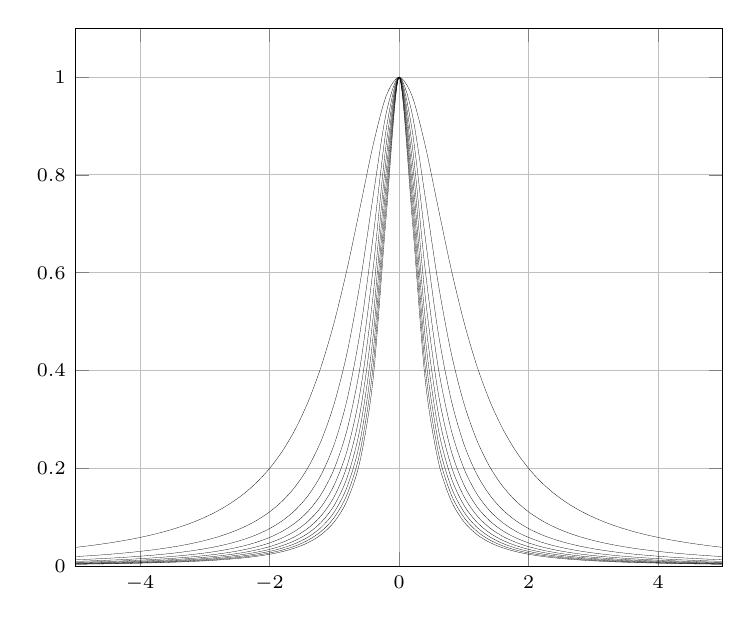
\begin{tikzpicture}
            \begin{axis}[domain=-5:5, restrict y to domain=0:1,
                xmin=-5, xmax=5, ymin=0, ymax=1.1, grid=both,
                tick label style={font=\scriptsize}, xscale=1.2, yscale=1.2]
                \addplot[samples=51,smooth,ultra thin] {1/(1 + 2*x^2)};
                \addplot[samples=51,smooth,ultra thin] {1/(1 + 3*x^2)};
                \addplot[samples=51,smooth,ultra thin] {1/(1 + 4*x^2)};
                \addplot[samples=51,smooth,ultra thin] {1/(1 + 1*x^2)};
                \addplot[samples=51,smooth,ultra thin] {1/(1 + 5*x^2)};
                \addplot[samples=51,smooth,ultra thin] {1/(1 + 6*x^2)};
                \addplot[samples=51,smooth,ultra thin] {1/(1 + 7*x^2)};
                \addplot[samples=51,smooth,ultra thin] {1/(1 + 8*x^2)};
                \addplot[samples=51,smooth,ultra thin] {1/(1 + 9*x^2)};
                \addplot[samples=51,smooth,ultra thin] {1/(1 + 10*x^2)};
            \end{axis}
        \end{tikzpicture}
    \end{figure}
\end{solution}

\subsection{Metryka Czebyszewa}
Weźmy pewną dwuargumentową funkcję zdefiniowąną jako
\[ d_c(f, g) = \sup_{x\in X}\left|f(x) - g(x)\right|. \]
Można udowodnić, że funkcja $d_c$ jest metryką (zwaną metryką Czebyszewa). Jako argumenty przyjmuje dwie funkcja zdefiniowane na tej samej dziedzinie $X$.

\begin{theorem}
    \label{t:uniform convergence iff metric = 0}
    Jeśli każda funkcja ciągu funkcyjnego $(f_n(x))$ jest ograniczona, to
    \[ f_n \rightrightarrows f \Longleftrightarrow \lim_{n\lthen\infty}d_c(f_n, f) = 0 .\]
\end{theorem}

\begin{example}
    Zbadaj zbieżność punktową i jednostajną ciągu funkcyjnego
    \[ f_n(x) = \frac{x^n}{1 + x^n} \]
    na przedziale $[2, \infty)$.
\end{example}
\begin{solution}
    Mamy
    \[ \lim_{n\lthen\infty} \frac{x^n}{1 + x^n} = 1 \equiv f, \]
    więc ciąg jest zbieżny punktowo do funkcji ciągłej, możemy zatem sprawdzić, czy zbiega do niej jednostajnie.
    \[ \lim_{n\lthen\infty}\sup_{x\in X} \left|\frac{x^n}{1 + x^n} - 1\right| = \lim_{n\lthen\infty}\sup_{x\in X} \left(1 - \frac{x^n}{1 + x^n}\right)\]
    Obliczmy supremum danej funkcji.
    \[ \ddx \left(1 - \frac{x^n}{1 + x^n}\right) = \frac{nx^{n-1}(1 + x^n) - x^n(nx^{n-1})}{\left(1 + x^n\right)^2} = \frac{nx^{n-1}}{\left(1 + x^n\right)^2} \]
    Pochodna zawsze jest dodatnia, więc supremum będzie przy $x \lthen \infty$. Mamy
    \[ \lim_{n\lthen\infty}\sup_{x\in X} \left(1 - \frac{x^n}{1 + x^n}\right) = \lim_{n\lthen\infty}\lim_{x\lthen\infty} \left(1 - \frac{x^n}{1 + x^n}\right) = \lim_{n\lthen\infty} \left(1 - 1\right) = 0, \]
    więc dany ciąg jest zbieżny jednostajnie.
\end{solution}

\begin{example}
    Zbadaj zbieżność punktową i jednostajną ciągu funkcyjnego
    \[ f_n(x) = \frac{nx}{n^2 + x^2} \]
    na zbiorze $\RR$.
\end{example}
\begin{solution}
    Mamy
    \[ \lim_{n\lthen\infty} \frac{nx}{n^2 + x^2} = \lim_{n\lthen\infty} \frac{x}{n} = 0 \equiv 0, \]
    więc ciąg jest zbieżny punktowo do funkcji ciągłej, możemy zatem sprawdzić, czy zbiega do niej jednostajnie.
    \[ \lim_{n\lthen\infty}\sup_{x\in X} \left|\frac{nx}{n^2 + x^2}\right| = \lim_{n\lthen\infty}\sup_{x\in X} \left(\frac{nx}{n^2 + x^2}\right) \]
    Obliczmy supremum danej funkcji.
    \[ \ddx \left(\frac{nx}{n^2 + x^2}\right) = \frac{n(n^2 + x^2) - nx(2x)}{\left(n^2 + x^2\right)^2} = \frac{n^3 - nx^2}{\left(n^2 + x^2\right)^2} \]
    Pochodna zeruje się, gdy
    \[ n^3 = nx^2 \implies x = \pm n, \]
    więc supremum będzie przy $x = n$. Mamy
    \[ \lim_{n\lthen\infty}\frac{n^2}{n^2 + n^2} = \frac{1}{2}, \]
    więc dany ciąg nie jest zbieżny jednostajnie.
\end{solution}

\begin{theorem}[o różniczkowalności granicy ciągu funkcyjnego]
    \label{t:differentiable limit}
    Jeśli każda funkcja ciągu funkcyjnego $(f_n(x))$ jest różniczkowalna, ciąg $(f_n)$ jest zbieżny, a ciąg $(f_n')$ zbieżny jednostajnie, to dla każdego $x \in X$ zachodzi
    \[ \left(\lim_{n\lthen\infty} f_n(x)\right)' = \lim_{n\lthen\infty} \left(f_n'(x)\right). \]
\end{theorem}

\begin{theorem}[o całkowalności granicy ciągu funkcyjnego]
    \label{t:integrable limit}
    Jeśli każda funkcja ciągu funkcyjnego $(f_n(x))$ jest całkowalna, a ciąg $(f_n)$ jest zbieżny jednostajnie, to dla każdych $x_1, x_2 \in X$ zachodzi
    \[ \int_{x_1}^{x_2}\left(\lim_{n\lthen\infty} f_n(x)\right) \d x = \lim_{n\lthen\infty} \left(\int_{x_1}^{x_2} f_n(x) \d x\right). \]
\end{theorem}